\documentclass[12pt,letter]{article}
\usepackage{geometry}\geometry{top=0.75in}
\usepackage{amsmath}
\usepackage{amssymb}
\usepackage{mathtools}
\usepackage{xcolor} % Color words
\usepackage{cancel} % Crossing parts of equations out
\usepackage{tikz}       % Drawing 
\usepackage{pgfplots}   % Other plotting
\usepgfplotslibrary{colormaps,fillbetween}
\usepackage{placeins}   % Float barrier
\usepackage{hyperref}   % Links
\usepackage{tikz-qtree} % Trees
\usepackage{graphicx}
\usepackage{subcaption}
\usepackage{multicol}
\usepackage{graphicx}   % For graphics
\usepackage{parcolumns}
\usepackage{listings}   % lstlisting
\usepackage{pdfpages}

\begin{document}
\title{CIS 551: Databases Final Project\\
\large Database of Climbing Routes}
\author{Steven Walton}
\maketitle
In this database we try to store information relevant to climbers when seeking
out routes to climb. We also give climbers the ability to store which climbs
they have done and to rate the climbs, both in difficulty and how much they
enjoy it. 

Information that we find relevant to climbers include the location of the routes
-- including the global location, what state it is in, and what climbing area it
is (e.g. Smith Rock or Red Stone) -- the difficulty of the climb, the type of
climb, how other climbers think the climb is (``likeability"), a description of
how to get there (approach), and a description of the climb itself, will be
available and several attributes will be adjustable for climbers. This
adjustable data will include climbers being able to vote on the difficulty of
the climb, how much they like it, and allows users to upload pictures.
Attributes like climbing difficulty and ``likeability" are subjective and
therefore it is best to aggregate this data and display the average result to
users. Additionally, users will be able to submit new routes.

A single climbing route can be composed of one or more pitches, which are half
the length of a standard rope. A route's overall difficulty is determined by the
highest difficulty rating of a single pitch, but information about individual
pitch difficulty is given so that climbers can best determine how to take breaks
and if they have adequate endurance for the climb. A pitch may be shared between
multiple routes. Some routes may be a single pitch, where a climber can then
just lower back to the ground. Other routes may continue from that pitch into a
more challenging route, or multiple routes my cross paths and share pitches.
Additionally, climbers need information about what gear they need for the climb.
There are three main subtypes: top-rope, sport, and trad. 

We will be using the American standard of the Yosemite Decimal System to express
the difficulty of climb. This
database will only consider climbs that require a rope, which means that the
leading integer value will always begin with a ``5". The decimal values range
from 1 (5.1) to 15 (5.15). Because of this we will only consider the range 1 to
15 given in a climbing rating and treat these values as integers.  Difficulties
above a 5.10 have sub alphabetic classifications ranging from ``a" to ``d", i.e.
5.10a, 5.10b, 5.10c, 5.10d express the entire range of 5.10 climbs.  These
alphabetic classifications will be expressed as the decimal representations
within the database with a value of 0.25 each. In this manner we can express an
average between values that climbers rank. For example, one climber may rate a
pitch as a 5.12a and another climber can rate the pitch as a 5.11c. These would
respectively by 12.0 and 11.5, respectively, giving an average rating of 11.75,
which will be converted to a 5.11d rating. We will use a ceiling function for
the averages, so that we error on the side of assigning a more difficult rating
to a pitch. Likeability of the climb will be expressed in the range of 1 to 10,
and the floor of the average rating will be displayed.

With this information climbers will be able to determine which routes that they
want to climb and what gear to bring. Climbers will also be able to use this
database to search out climbs that they may find enjoyable. The website will
enable climbers to search through the database, including: finding routes by
area, finding routes by difficulty, likeability, number of pitches, or a
combination of these. Additionally climbers will be able to navigate through the
website based on the hierarchy of the routes. This hierarchy is the hemisphere,
country, state, area, and route. These pages will themselves have information
and links to the next element in the hierarchy. For example by clicking on Area
climbers will be presented with a list of routes in that area or if a climber
clicks on a country they will be given a list of states that have routes in the
database. Pitches will not be given their own page. 

\FloatBarrier
\begin{figure}[ht!]
    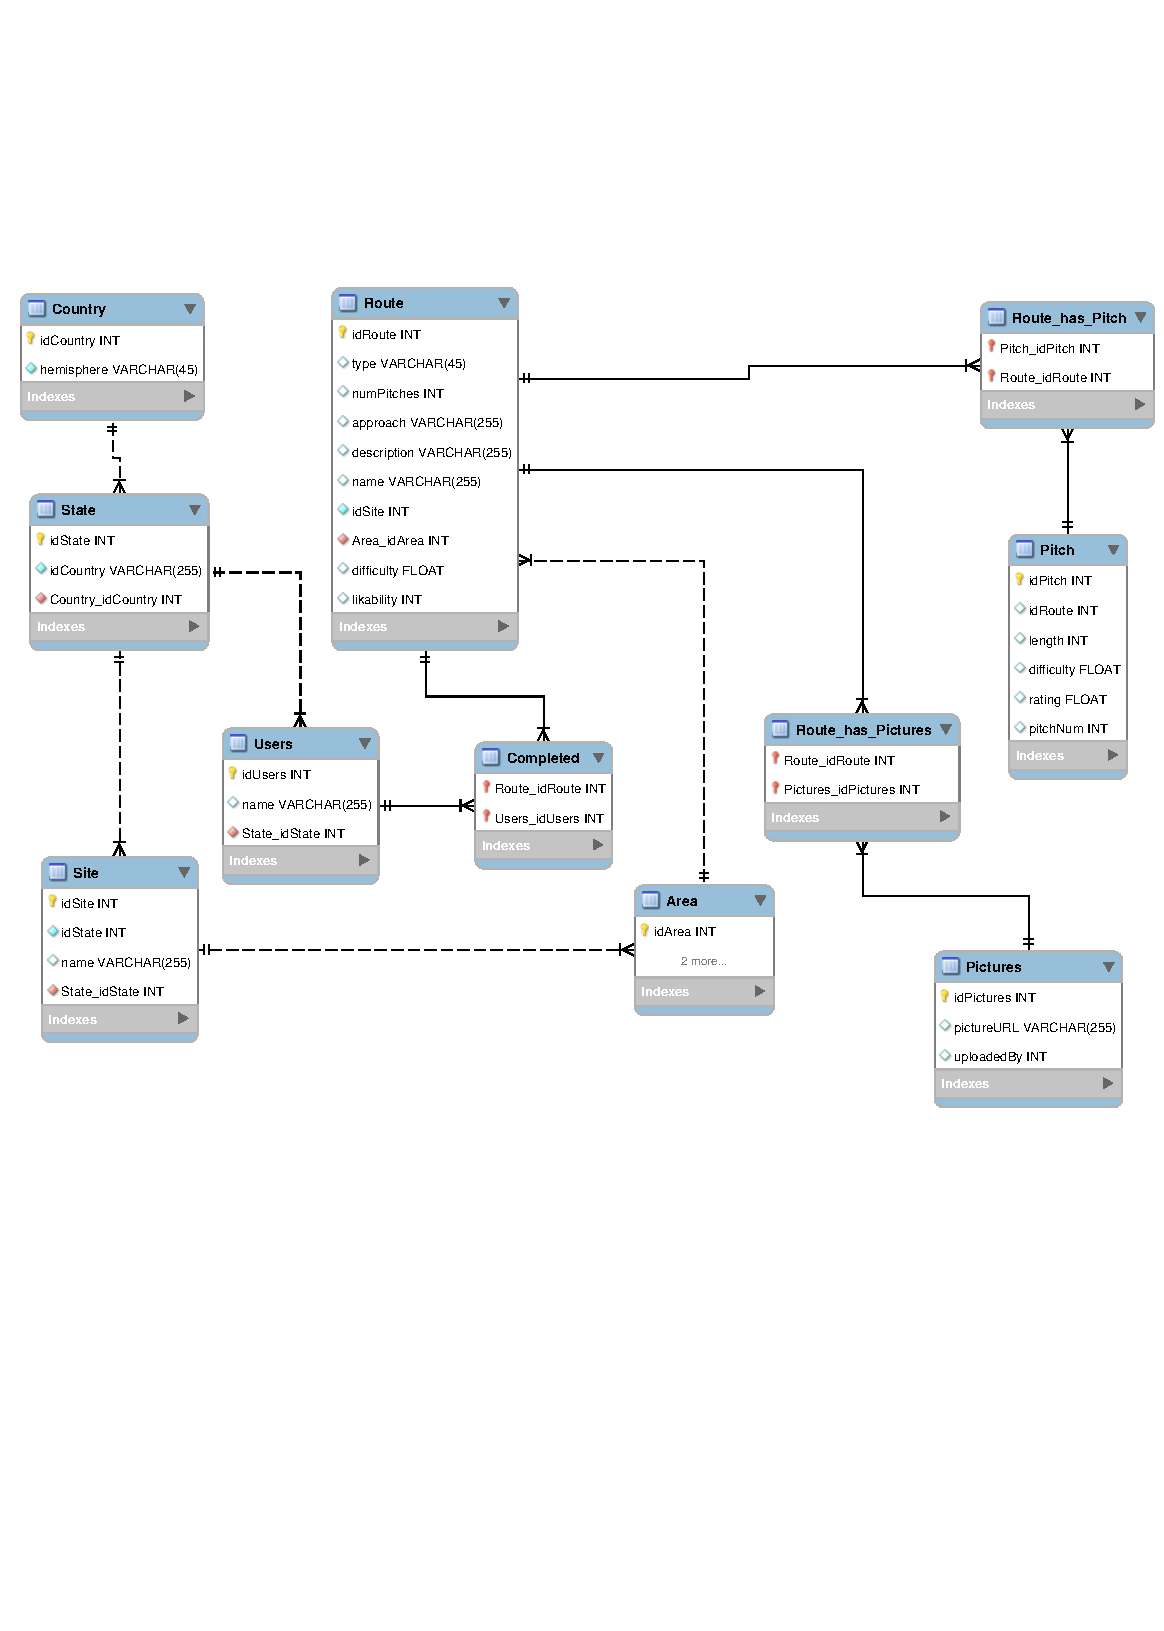
\includegraphics[trim={0 8.5cm 0 4.5cm},clip, width=\textwidth]{ER_Diagram.pdf}
\end{figure}
\end{document}
